\PassOptionsToPackage{unicode=true}{hyperref} % options for packages loaded elsewhere
\PassOptionsToPackage{hyphens}{url}
%
\documentclass[
]{article}
\usepackage{lmodern}
\usepackage{amssymb,amsmath}
\usepackage{ifxetex,ifluatex}
\ifnum 0\ifxetex 1\fi\ifluatex 1\fi=0 % if pdftex
  \usepackage[T1]{fontenc}
  \usepackage[utf8]{inputenc}
  \usepackage{textcomp} % provides euro and other symbols
\else % if luatex or xelatex
  \usepackage{unicode-math}
  \defaultfontfeatures{Scale=MatchLowercase}
  \defaultfontfeatures[\rmfamily]{Ligatures=TeX,Scale=1}
\fi
% use upquote if available, for straight quotes in verbatim environments
\IfFileExists{upquote.sty}{\usepackage{upquote}}{}
\IfFileExists{microtype.sty}{% use microtype if available
  \usepackage[]{microtype}
  \UseMicrotypeSet[protrusion]{basicmath} % disable protrusion for tt fonts
}{}
\makeatletter
\@ifundefined{KOMAClassName}{% if non-KOMA class
  \IfFileExists{parskip.sty}{%
    \usepackage{parskip}
  }{% else
    \setlength{\parindent}{0pt}
    \setlength{\parskip}{6pt plus 2pt minus 1pt}}
}{% if KOMA class
  \KOMAoptions{parskip=half}}
\makeatother
\usepackage{xcolor}
\IfFileExists{xurl.sty}{\usepackage{xurl}}{} % add URL line breaks if available
\IfFileExists{bookmark.sty}{\usepackage{bookmark}}{\usepackage{hyperref}}
\hypersetup{
  pdftitle={Monthly Report of Peak Shaving project on Fort William TS Power Station},
  pdfborder={0 0 0},
  breaklinks=true}
\urlstyle{same}  % don't use monospace font for urls
\usepackage[margin=1in]{geometry}
\usepackage{longtable,booktabs}
% Allow footnotes in longtable head/foot
\IfFileExists{footnotehyper.sty}{\usepackage{footnotehyper}}{\usepackage{footnote}}
\makesavenoteenv{longtable}
\usepackage{graphicx,grffile}
\makeatletter
\def\maxwidth{\ifdim\Gin@nat@width>\linewidth\linewidth\else\Gin@nat@width\fi}
\def\maxheight{\ifdim\Gin@nat@height>\textheight\textheight\else\Gin@nat@height\fi}
\makeatother
% Scale images if necessary, so that they will not overflow the page
% margins by default, and it is still possible to overwrite the defaults
% using explicit options in \includegraphics[width, height, ...]{}
\setkeys{Gin}{width=\maxwidth,height=\maxheight,keepaspectratio}
\setlength{\emergencystretch}{3em}  % prevent overfull lines
\providecommand{\tightlist}{%
  \setlength{\itemsep}{0pt}\setlength{\parskip}{0pt}}
\setcounter{secnumdepth}{-2}
% Redefines (sub)paragraphs to behave more like sections
\ifx\paragraph\undefined\else
  \let\oldparagraph\paragraph
  \renewcommand{\paragraph}[1]{\oldparagraph{#1}\mbox{}}
\fi
\ifx\subparagraph\undefined\else
  \let\oldsubparagraph\subparagraph
  \renewcommand{\subparagraph}[1]{\oldsubparagraph{#1}\mbox{}}
\fi

% set default figure placement to htbp
\makeatletter
\def\fps@figure{htbp}
\makeatother

\usepackage{float}

\title{Monthly Report of Peak Shaving project on Fort William TS Power Station}
\author{}
\date{\vspace{-2.5em}2021-April}

\begin{document}
\maketitle

\hypertarget{overview}{%
\section{Overview}\label{overview}}

This monthly report analyzes the Peak Shaving system of Fort William TS
power station during 2018-April. This report contains four sections:
First, the graphical results of peak shaving activities of power
consumption. Second, the numerical results peak shaving activities of
power consumption and expected bill saving. Third, the monthly
performance of energy forecasting models. Four, detailed peak shaving
activities of the highest five peak days during this month.

\hypertarget{the-graphical-results-of-peak-shaving}{%
\section{The graphical results of Peak
Shaving}\label{the-graphical-results-of-peak-shaving}}

Figure (\ref{fig:fig1}) shows a monthly forecasting graph. The black
line describes the actual power consumption curve; the red line
describes the prediction curve and the yellow line describes the battery
discharging period set by the predicted peak.

\begin{figure}[H]
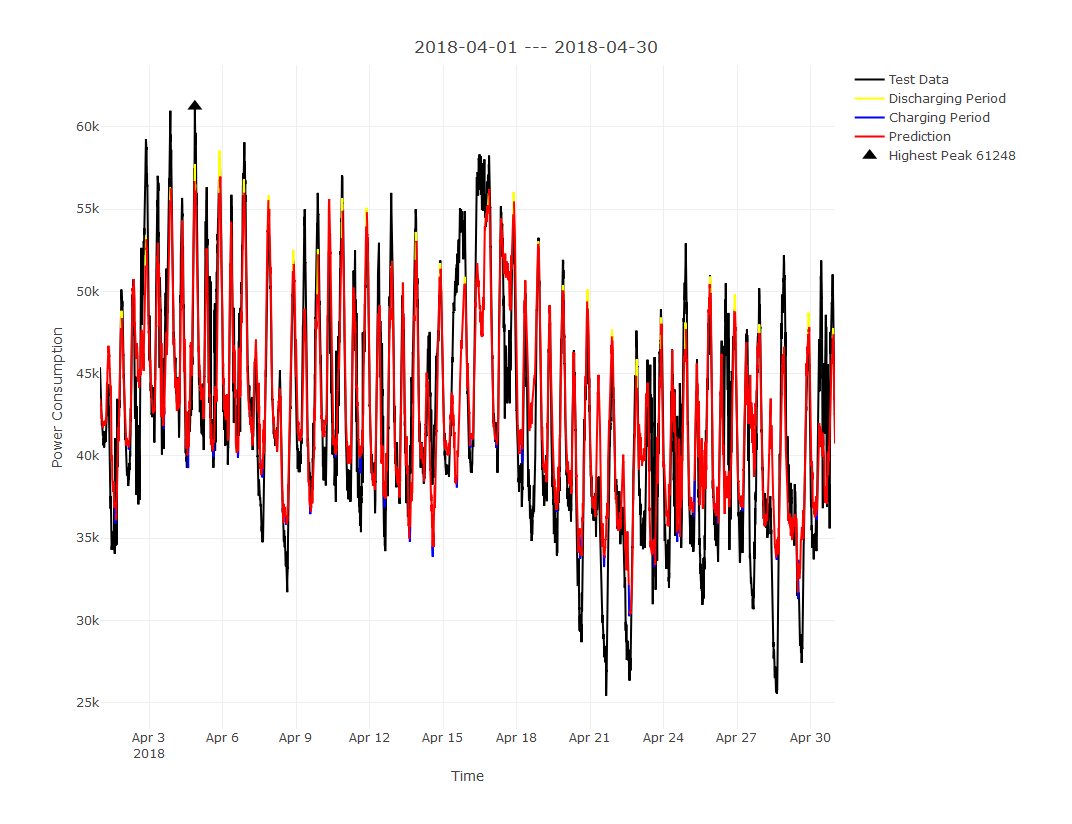
\includegraphics[width=1\linewidth]{monthly} \caption{Monthly forecasting graph\label{fig1}}\label{fig:fig1}
\end{figure}

Figure (\ref{fig:fig2}) shows a comparison of the expected power
consumption curve(black) and after the peak-shaving curve(red).
According to figure (\ref{fig:fig2}), The highest peak of power
consumption of the month is reduced from {61248}kW ({2018-04-04
20:55:00}) to { 59635.2}kW ({ 2018-04-04 21:50:00}). Figure
(\ref{fig:fig3}) shows the detailed peak shaving result of the highest
peak of the month which is in 2018-04-04.

\begin{figure}[H]
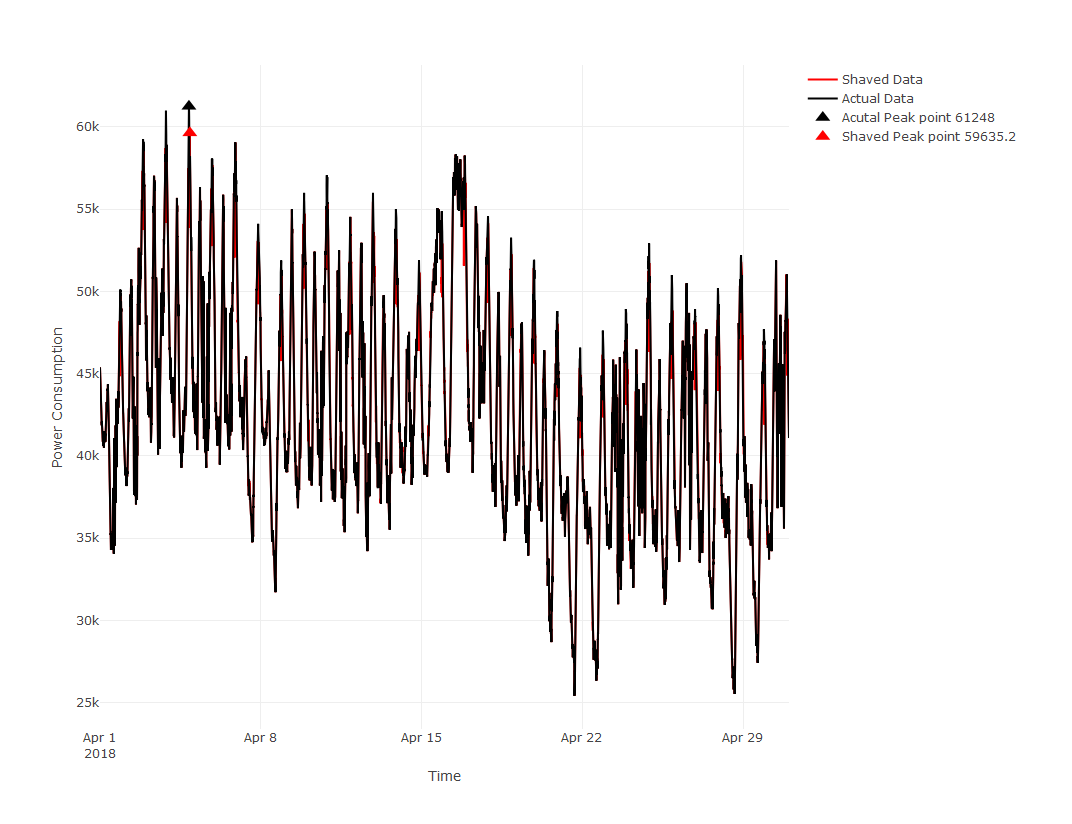
\includegraphics[width=1\linewidth]{monthly_shaved} \caption{Monthly Peak Shaving Activies graph\label{fig2}}\label{fig:fig2}
\end{figure}

\begin{figure}[H]
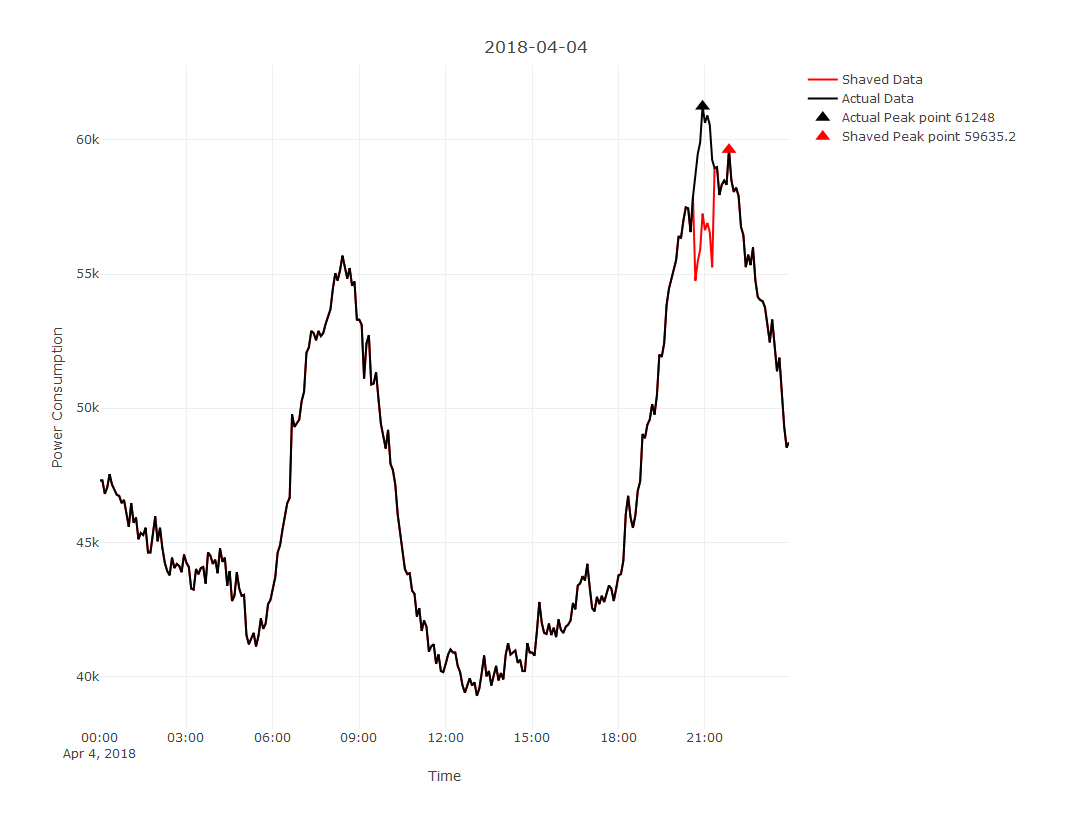
\includegraphics[width=1\linewidth]{daily} \caption{Highest peak day\label{fig3}}\label{fig:fig3}
\end{figure}

\hypertarget{the-digital-results-of-peak-shaving}{%
\section{The digital results of Peak
shaving:}\label{the-digital-results-of-peak-shaving}}

As shown in Table (\ref{tab:table1}), the expected peak of power
consumption is {61248}kW occur at {2018-04-04 20:55:00}. After the
peak-shaving activities, the highest peak of this month reduces to {
59635.2}kW at { 2018-04-04 21:50:00}. The monthly energy purchasing cost
reduces from \${30624} to \${29817.6}, which saves \${806.4}.

\begin{longtable}[]{@{}lllr@{}}
\caption{Monthly Results Table}\tabularnewline
\toprule
Parameter & April Expected Peak & April Shaved Peak & Total
Reduction\tabularnewline
\midrule
\endfirsthead
\toprule
Parameter & April Expected Peak & April Shaved Peak & Total
Reduction\tabularnewline
\midrule
\endhead
Power Consumption(kW) & 61248 & 59635.2 & 1612.8\tabularnewline
Billing(\$) & 30624 & 29817.6 & 806.4\tabularnewline
\bottomrule
\end{longtable}

\hypertarget{the-performance-of-the-forecasting-system}{%
\section{The performance of the forecasting
system:}\label{the-performance-of-the-forecasting-system}}

In this energy forecasting system, we combine four different models.
Table (\textbackslash{}ref\{tab:table2)) show the monthly performance of
each model. There are four machine learning algorithms in total: Cubist,
Xgboost, (feedforward) Neural Network and LSTM (Long short-term memory).
The ensemble model combines all four algorithms and battery discharging
events base on the ensemble model.

Relative root mean square error (rRMSE), which is RMSE divided by the
average power consumption of tested day, between 1:00 pm to 12:00 pm to
represent the performance of a model on the ability of prediction peak
period. In the following formula, n represent number of data between
1:00 pm to 12:00 pm, y\textsubscript{i} and x\textsubscript{i} are the
prediction and real power consumption receptively.

\begin{align}
rRMSE = \frac{1\sqrt{(\frac{1}{n})\sum_{i=1}^{n}(y_{i} - x_{i})^{2}}}{\frac{1}{n}\sum_{i=1}^{n}x_{i}}
\end{align}

Average Peak time error represent the mean of daily time different of
expected peak time and predicted peak time. Pecentage of daily peak
shaved represent the pecentage of days which discharging period coverd
actual peak time in this month. For example, 0.8 mean this peak shaving
system successfully shaved 80\% of daily peak in this month.

\begin{longtable}[]{@{}lrrrrrr@{}}
\caption{Monthly Models Performance}\tabularnewline
\toprule
Parameter & Cubist & Xgboost & Random Forest & Nerual Network & LSTM &
Ensemble System\tabularnewline
\midrule
\endfirsthead
\toprule
Parameter & Cubist & Xgboost & Random Forest & Nerual Network & LSTM &
Ensemble System\tabularnewline
\midrule
\endhead
rRMSE & 0.10 & 0.09 & 0.09 & 0.10 & 0.10 & 0.08\tabularnewline
Average Peak time error & 44.68 & 39.35 & 29.52 & 26.13 & 20.16 &
27.48\tabularnewline
percentage of daily peak shaved & 0.71 & 0.68 & 0.84 & 0.87 & 0.90 &
0.94\tabularnewline
\bottomrule
\end{longtable}

The accuracy of energy forecasting on the highest peak of the month is
an important factor to measure the performance of each model. Figure
(\ref{fig:fig4}) show the performance of each model on the day with
highest peak.

\begin{figure}[H]
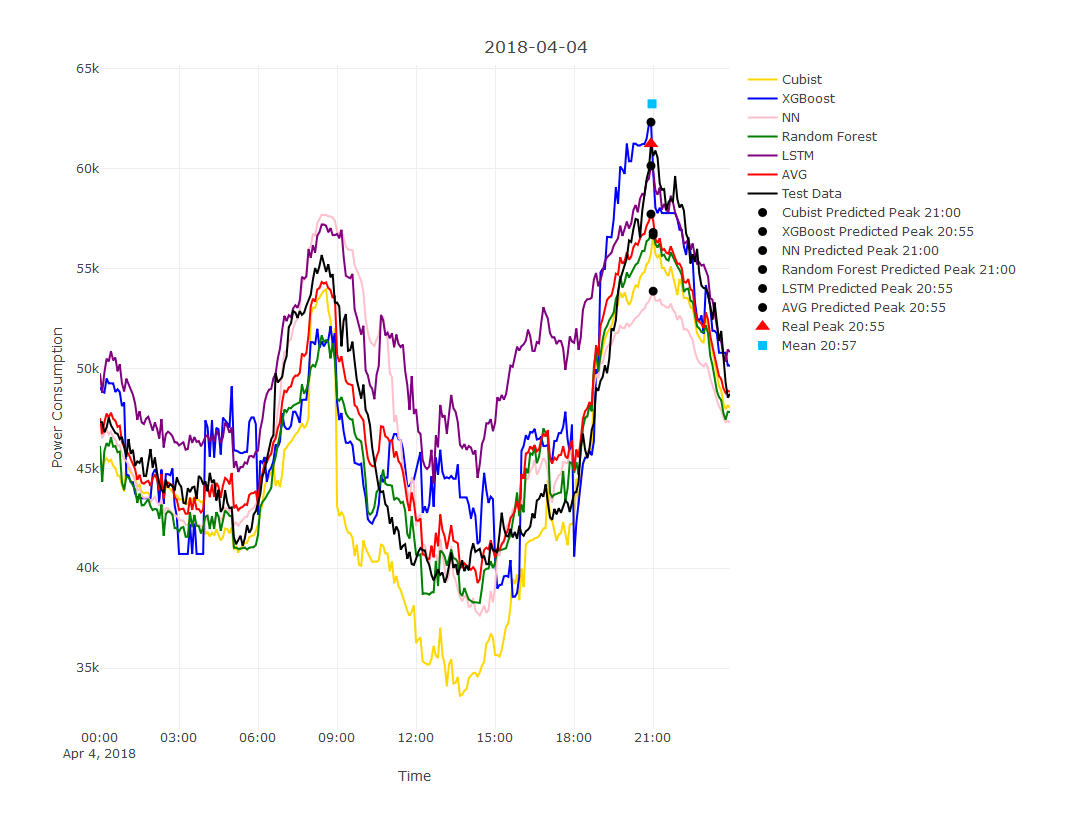
\includegraphics[width=1\linewidth]{model_performance} \caption{Daily Models Performance\label{fig4}}\label{fig:fig4}
\end{figure}

\hypertarget{detailed-report}{%
\section{Detailed report:}\label{detailed-report}}

Top five highest peak days are shown in Figure
(\ref{fig:day1})(\ref{fig:day2}) respectively.

\begin{figure}
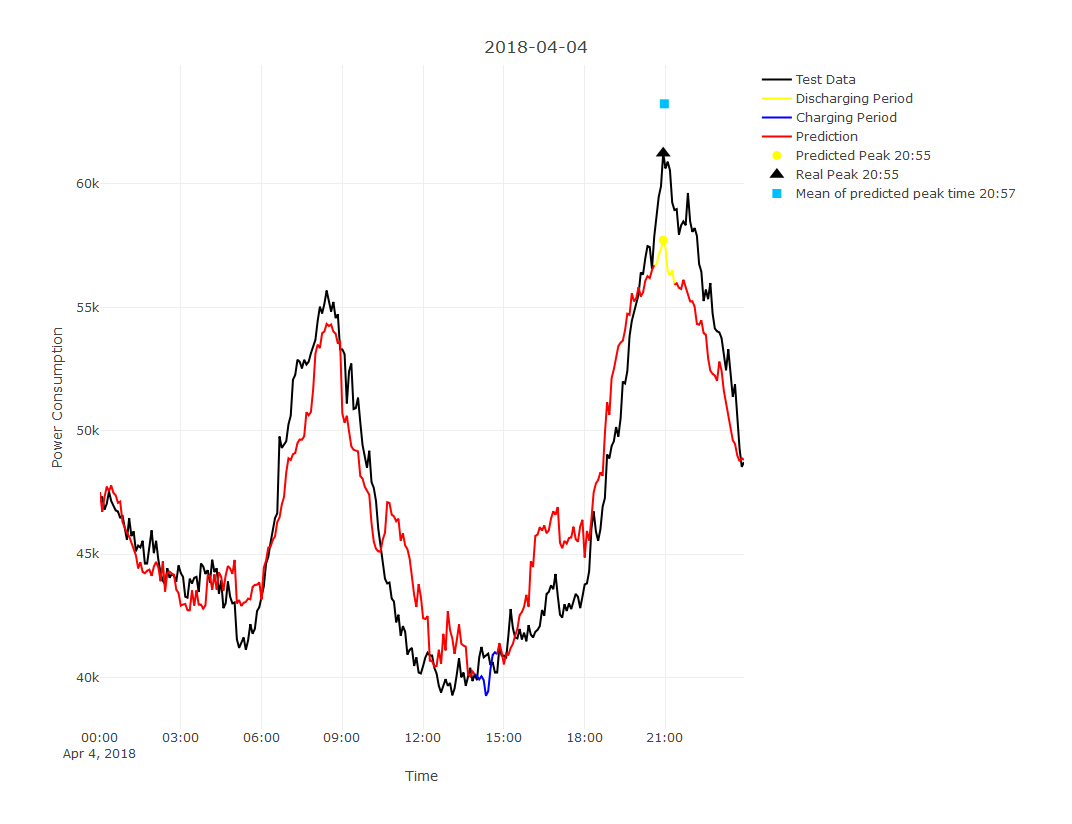
\includegraphics[width=1\linewidth]{day1} \caption{Highest Peak day\label{day1}}\label{fig:day1}
\end{figure}
\begin{figure}
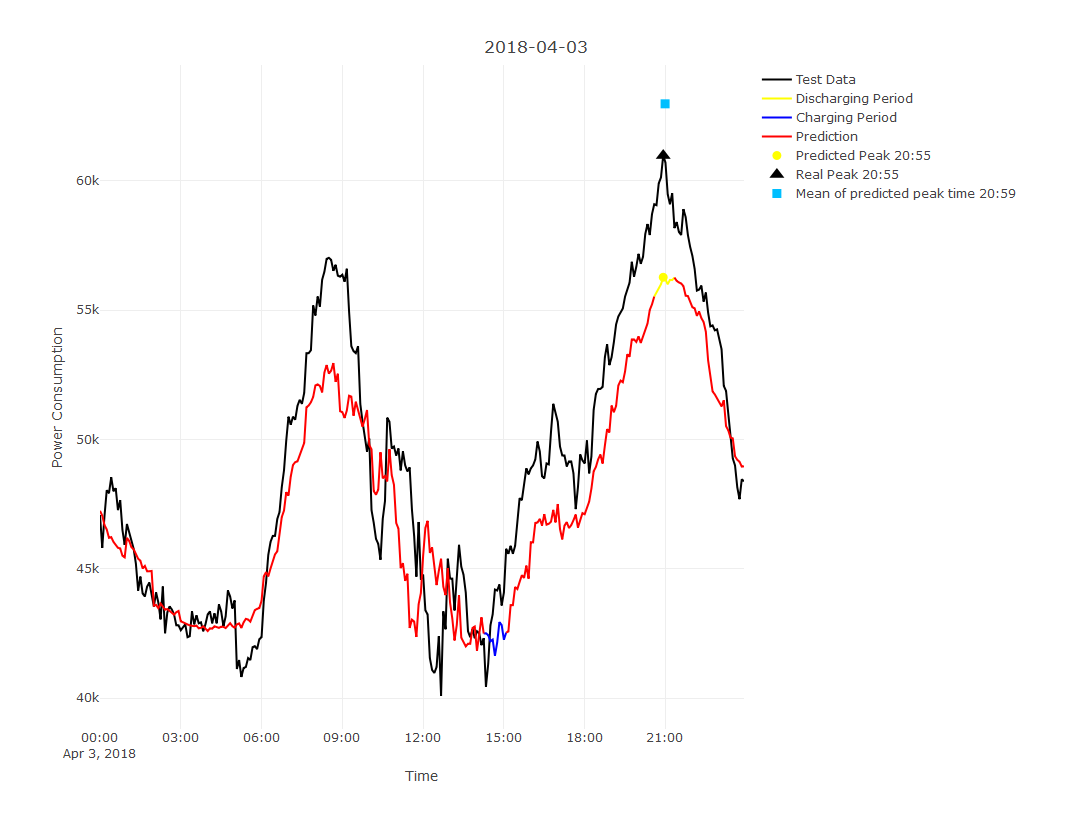
\includegraphics[width=1\linewidth]{day2} \caption{2nd Highest Peak day\label{day2}}\label{fig:day2}
\end{figure}

\begin{figure}
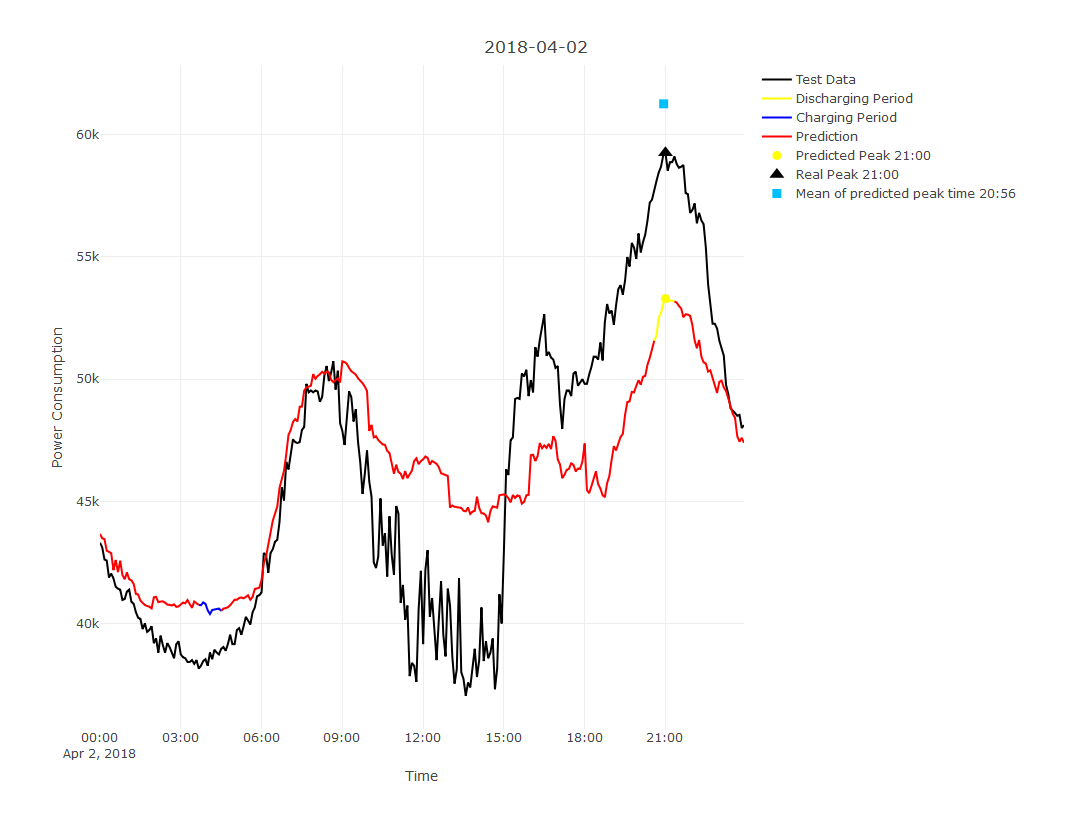
\includegraphics[width=1\linewidth]{day3} \caption{3rd Highest Peak day\label{day3}}\label{fig:day3}
\end{figure}

\begin{figure}
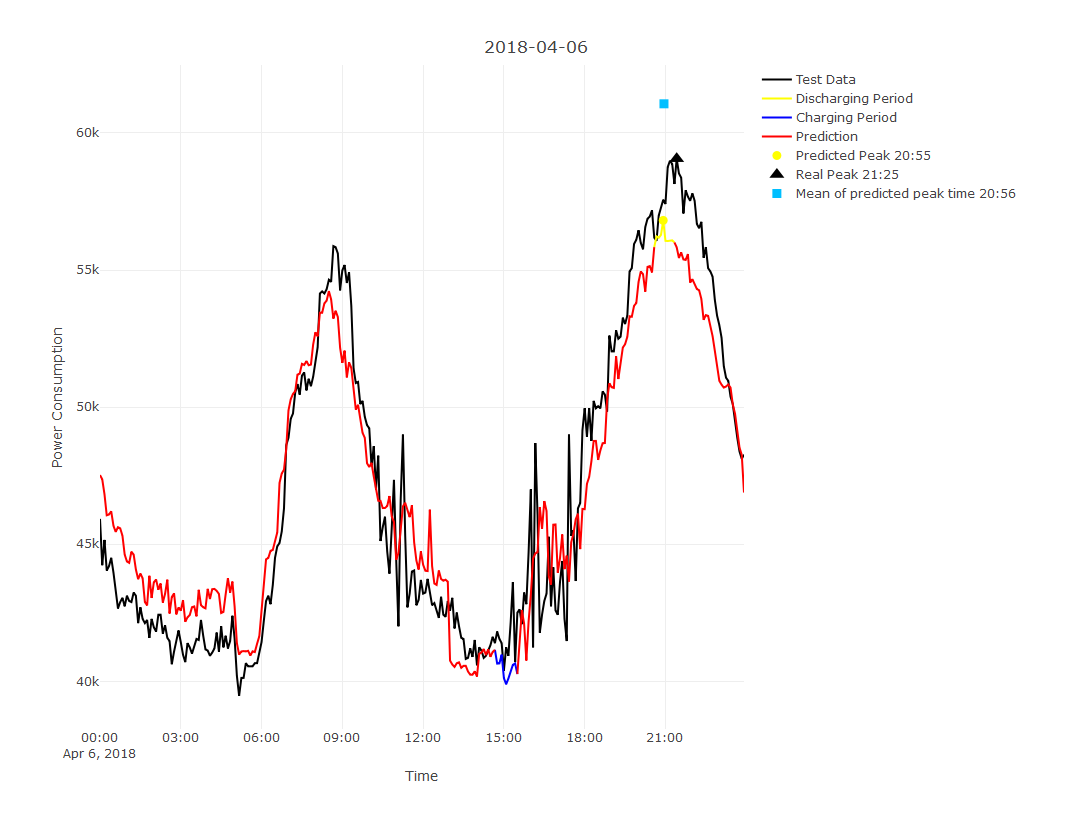
\includegraphics[width=1\linewidth]{day4} \caption{4th Highest Peak day\label{day4}}\label{fig:day4}
\end{figure}

\begin{figure}
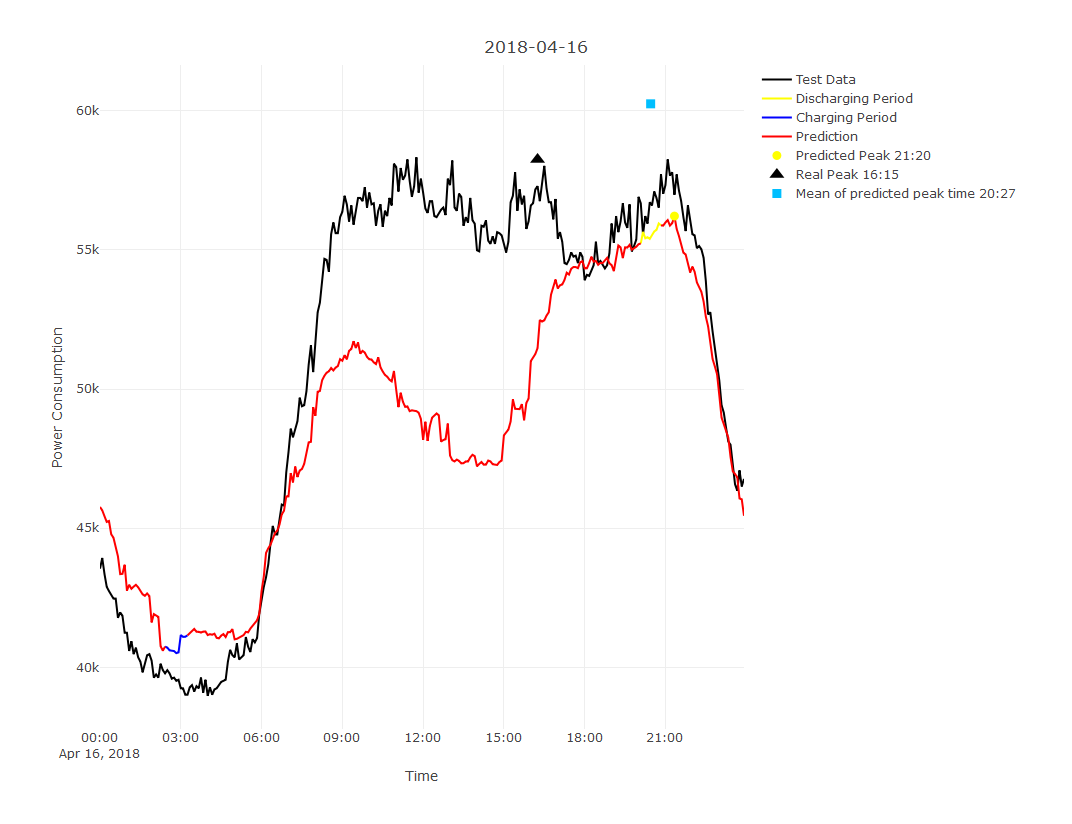
\includegraphics[width=1\linewidth]{day5} \caption{5th Highest Peak day\label{day5}}\label{fig:day5}
\end{figure}

\end{document}
